\documentclass[a4paper,12pt]{article}
\usepackage{a4wide}
\usepackage{acronym}
\usepackage{graphicx}
\usepackage[title,titletoc,toc]{appendix}


\begin{document}

\begin{center}
{\LARGE\bf Travelling Thief Problem}\\
\vspace{0.5cm}
{\Large\bf Evolutionary Computation}\\
\vspace{1cm}
Prepared by William Reid, Matthew Hart, Samantha Peachey \& Alec Bellati\\
\vspace{1cm}
School of Computer Science,\\
The University of Adelaide\\
\vspace{1cm}
\today
\end{center}

\vspace{1cm}
\section*{Exercise 5}


\newpage
\section{Test Parameters}
Definitions:
\begin{itemize}
	\item {\bf Knapsack Seed:} The algorithm allows for various methods to seed the knapsack. The ``seed'' is the starting packing of the knapsack and can greatly affect the final result. Seed 2 chooses items based on their profit-to-weight ratio, while seed 4 randomly picks items.
	\item {\bf TSP Choice:} To account for extendibility, this algorithm not only considers just the packing of the knapsack, but may also consider changes to the TSP tour. Choice 1 simple uses the supplied linkern tour, where as choice 2 will use our best TSP algorithm from assignment 1.
	\item {\bf Generations:} Number of times to perform the algorithm on the knapsack (knapsack packing is retained for the next generation, it is not re-seeded).
	\item {\bf Iterations:} Number of times to replace a randomly chosen item in the knapsack with the current item. A value of ``ALL'' implies every item in the knapsack will be replaced to find the optimal position of the current item.
	\item {\bf Items to be considered:} Number of items to be placed in the knapsack to evaluate. A value of ``ALL'' implies every item not currently contained within the knapsack will be considered.
\end{itemize}

\begin{figure}[h]
\centering
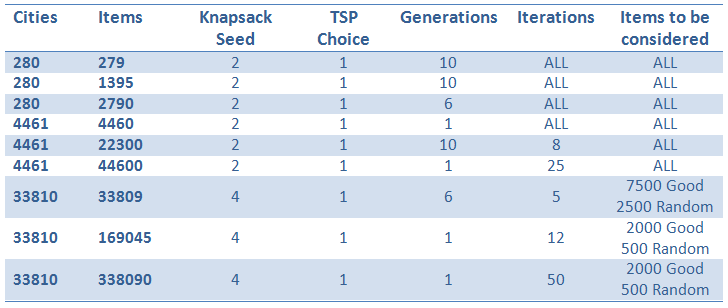
\includegraphics[width=\linewidth]{ParamsTable.png}
\end{figure}

\newpage
\section{Results}
For each instance, the algorithms mentioned in the table below were run 20 times and the result was obtained. In addition the execution time for the entire 20 runs was recorded. The timer was set-up independent of the Java classes and hence the minor fluctuations above the allocated 600 seconds (10 minutes) are due to the set-up and deallocation of the Java instances and do not imply a longer execution time of the algorithm.
\begin{figure}[h]
\centering
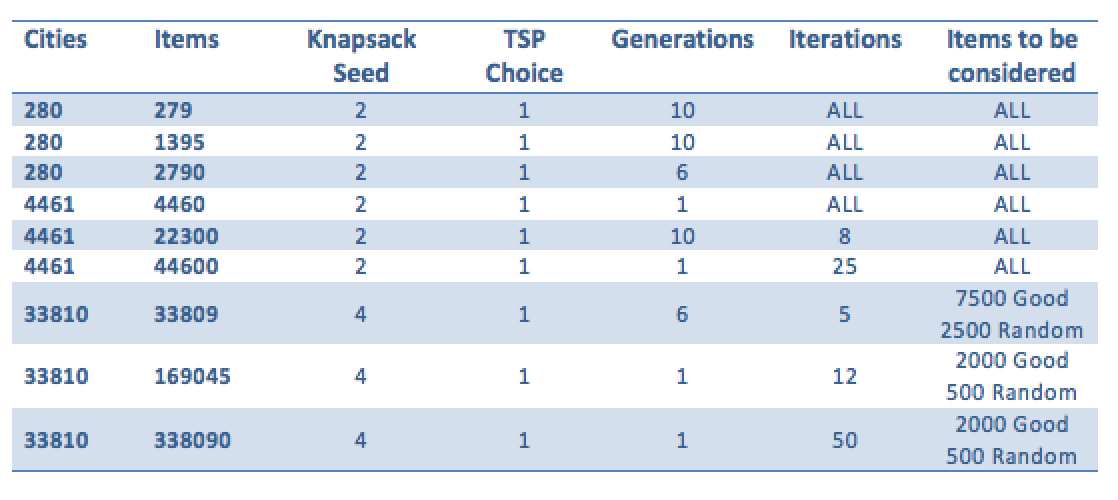
\includegraphics[width=\linewidth]{ResultsTable.png}
\end{figure}

\section{Conclusion}
The results shown in the previous section show that the Obsessive Packing algorithm can consistently obtain values equal to or higher then that of the \textit{Hill Climber} algorithm. Due to its intrinsic design, smaller data sets take slightly longer (apart from the the first). However as the instances grow larger,  the Obsessive Packing algorithm obtains a better result within the allocated and provided it could continue past the 10 minute limit, would also complete sooner then that of the hill climber algorithm.\\

The Obsessive Packing algorithm could be improved by considering changes to the TSP tour. Instances {\bf a280\_n1395} and {\bf a280\_n2790} appear to reach the optimal knapsack packing for the supplied tour, hence implying that modifying the TSP tour based on the knapsack may infact yield better results.

\end{document}
